
\section{\trSmaleCondition}
\label{sec:the-smale-condition}

让我们回到各\trCriticalPoint{}的\trStableManifold{}与\trUnstableManifold。

\subsection{\trStableManifold{}与\trUnstableManifold{}的例子}
\label{subsec:examples-stable-unstable}

下面就给出前文诸例中各\trCriticalPoint{}的\trStableManifold{}与\trUnstableManifold。

\emph{圆\trSphere{}上的高度。}

设 $a$ 为极小点、$b$ 为极大点。我们有
\[
W^s(a)=S^2-\{b\}\text{，}\qquad W^u(a)=\{a\}
\]
同理
\[
W^s(b)=\{b\}\text{，}\qquad W^u(b)=S^2-\{a\}
\]
（对每一个\trPseudogradient{}场皆然）。

\emph{\trTorus。}

我们先来看“内胎”\trTorus{}上的\trHeightFunction。设 $a$、$b$、$c$、$d$ 是按函数在这些点处所取值的大小排序后的诸\trCriticalPoint（\cref{fig:height-torus}）。这里使用的\trPseudogradient{}场无非就是\trTorus{}上由 $\RR^3$ 上的\trMetric{}所诱导的那个\trMetric{}下的\trGradient。$a$ 的\trStableManifold{}由一切下降到 $a$ 的点组成，也就是说，由图中那些终止于 $b$ 或 $c$ 的\trTrajectory{}的补集组成。因此 $W^s(a)$ \trHomeomorphic{}于一个\trOpen{}\trDisk。$b$ 的\trStableManifold{}由从 $c$ 出发、终止于 $b$ 的两条\trTrajectory{}组成，故 $W^s(b)$ \trDiffeomorphic{}于一个\trOpen{}区间。$c$ 的\trStableManifold{}也是如此，它由我们在图中看到的、从 $d$ 出发的那两条\trTrajectory{}组成。应当注意，在本例中（选这个例子正是出于这一原因），$c$ 的\trUnstableManifold{}与 $b$ 的\trStableManifold{}有两段\trOpen{}区间是公共的。\cref{fig:torus-square}则在一个正方形中描出了同一函数的几个\trLevelSet，这就解出了上一章提出的一个练习；图中还画出了\trGradient{}的几条\trTrajectory。

\setcounter{figure}{9}%
\begin{figure}[htbp]
\begin{minipage}[b]{0.40\textwidth}
\centering
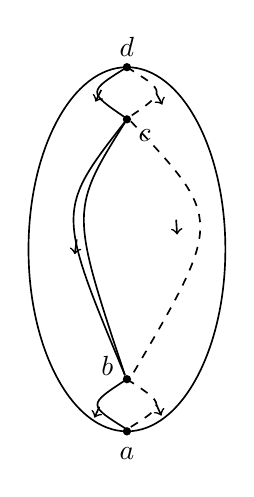
\begin{tikzpicture}[line width=0.6pt,scale=1.25]
  \draw (0,0) ellipse (1.0 and 1.85);
  \fill (0,1.85) circle (1.2pt);
  \fill (0,1.32) circle (1.2pt);
  \fill (0,-1.32) circle (1.2pt);
  \fill (0,-1.85) circle (1.2pt);
  \draw (0,1.85) .. controls (-0.40,1.60) .. (-0.02,1.34);
  \draw[->] (-0.26,1.62) -- (-0.32,1.50);
  \draw[dashed] (0,1.85) .. controls (0.40,1.60) .. (0.02,1.34);
  \draw[->] (0.30,1.58) -- (0.36,1.47);
  \draw (0,1.32) .. controls (-0.72,0.4) .. (-0.02,-1.28);
  \draw (0,1.32) .. controls (-0.58,0.4) .. (-0.02,-1.28);
  \draw[->] (-0.51,0.1) -- (-0.53,-0.05);
  \draw[dashed] (0.04,1.30) .. controls (0.98,0.3) .. (0.04,-1.30);
  \draw[->] (0.50,0.30) -- (0.51,0.15);
  \draw (0,-1.32) .. controls (-0.40,-1.58) .. (0,-1.83);
  \draw[->] (-0.28,-1.60) -- (-0.33,-1.71);
  \draw[dashed] (0,-1.32) .. controls (0.40,-1.58) .. (0,-1.83);
  \draw[->] (0.30,-1.58) -- (0.35,-1.69);
  \node at (0,2.06) {$d$};
  \node at (0.18,1.16) {$c$};
  \node at (-0.20,-1.18) {$b$};
  \node at (0,-2.08) {$a$};
\end{tikzpicture}
\caption{\trTorus{}上的高度}
\label{fig:height-torus}
\end{minipage}\hfill
\begin{minipage}[b]{0.56\textwidth}
\centering
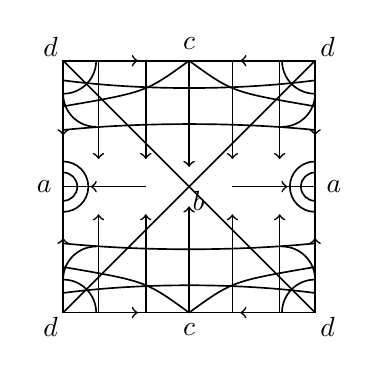
\begin{tikzpicture}[line width=0.6pt,scale=1.0]
  \draw (0,0) rectangle (3.2,3.2);
  \draw (0,1.6) -- (0.9,1.6); \draw[->] (1.05,1.6) -- (0.35,1.6);
  \draw (2.3,1.6) -- (3.2,1.6); \draw[->] (2.15,1.6) -- (2.85,1.6);
  \draw (1.6,3.2) -- (1.6,2.0); \draw[->] (1.6,2.15) -- (1.6,1.85);
  \draw (1.6,1.2) -- (1.6,0); \draw[->] (1.6,1.05) -- (1.6,1.35);
  \foreach \x in {0.45,1.05,2.15,2.75}{
    \draw (\x,3.2) -- (\x,2.5); \draw[->] (\x,2.5) -- (\x,1.95);
    \draw (\x,0) -- (\x,0.7); \draw[->] (\x,0.7) -- (\x,1.25);
  }
  \draw (1.6,1.6) -- (0,3.2);
  \draw (1.6,1.6) -- (3.2,3.2);
  \draw (1.6,1.6) -- (0,0);
  \draw (1.6,1.6) -- (3.2,0);
  \draw (0,1.92) arc (90:-90:0.32);
  \draw (0,1.78) arc (90:-90:0.18);
  \draw (3.2,1.92) arc (90:270:0.32);
  \draw (3.2,1.78) arc (90:270:0.18);
  \draw (1.6,3.2) .. controls (1.05,2.8) .. (0,2.62);
  \draw (1.6,3.2) .. controls (2.15,2.8) .. (3.2,2.62);
  \draw (1.6,0) .. controls (1.05,0.4) .. (0,0.58);
  \draw (1.6,0) .. controls (2.15,0.4) .. (3.2,0.58);
  \draw (0,2.95) .. controls (1.0,2.82) and (2.2,2.82) .. (3.2,2.95);
  \draw (0,2.32) .. controls (1.0,2.42) and (2.2,2.42) .. (3.2,2.32);
  \draw (0,0.88) .. controls (1.0,0.78) and (2.2,0.78) .. (3.2,0.88);
  \draw (0,0.25) .. controls (1.0,0.38) and (2.2,0.38) .. (3.2,0.25);
  \draw (0.42,3.2) arc (0:-90:0.42);
  \draw (0,2.78) arc (180:270:0.42);
  \draw (2.78,3.2) arc (180:270:0.42);
  \draw (3.2,2.78) arc (0:-90:0.42);
  \draw (0.42,0) arc (0:90:0.42);
  \draw (0,0.42) arc (180:90:0.42);
  \draw (2.78,0) arc (180:90:0.42);
  \draw (3.2,0.42) arc (0:90:0.42);
  \draw[->] (0.55,3.2) -- (0.95,3.2);
  \draw[->] (2.65,3.2) -- (2.25,3.2);
  \draw[->] (0.55,0) -- (0.95,0);
  \draw[->] (2.65,0) -- (2.25,0);
  \draw[->] (0,2.65) -- (0,2.25);
  \draw[->] (0,0.55) -- (0,0.95);
  \draw[->] (3.2,2.65) -- (3.2,2.25);
  \draw[->] (3.2,0.55) -- (3.2,0.95);
  \node at (-0.16,3.38) {$d$};
  \node at (1.6,3.42) {$c$};
  \node at (3.36,3.38) {$d$};
  \node at (-0.24,1.6) {$a$};
  \node at (3.44,1.6) {$a$};
  \node at (1.72,1.42) {$b$};
  \node at (-0.16,-0.18) {$d$};
  \node at (1.6,-0.22) {$c$};
  \node at (3.36,-0.18) {$d$};
\end{tikzpicture}
\caption{同一事物的另一种视角}
\label{fig:torus-square}
\end{minipage}
\end{figure}

对于我们在\trTorus{} $T^2$ 上遇到的另一个\trMorseFunction，情况就有些不同了，即
\[
f(x,y)=\cos(2\pi x)+\cos(2\pi y)\text{。}
\]

我们仍把两个\trExtremum{}记作 $a$ 与 $d$，把两个\trIndex{}为~1 的\trCriticalPoint{}记作 $b$ 与 $c$。\cref{fig:torus-again}画出了连接这两个\trCriticalPoint{}的诸条\trGradient{}线（这里我们用的是\trTorus{}上“平坦”\trMetric，也就是 $\RR^2$ 上通常的\trMetric{}下的\trGradient；可以看到，所论这些线与诸\trLevelSet{}构成真正的直角）。可以清楚地看到：$W^s(a)$ 是\trOpen{}正方形（也就是一个\trOpen{}\trDisk）；$W^s(b)$ 是一个\trOpen{}区间（即图中正方形的水平边），$W^u(b)$（竖直段）、$W^s(c)$（竖直边）与 $W^u(c)$（水平段）亦然；而 $W^s(d)$ 则缩成了 $\{d\}$。注意，$W^u(b)$ 与 $W^s(c)$ 不相交。

\begin{figure}[htbp]
\centering
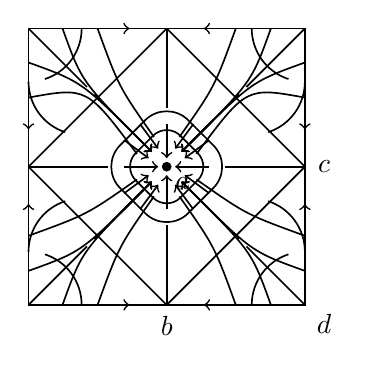
\begin{tikzpicture}[line width=0.6pt,scale=1.35]
  \draw (0,0) rectangle (2.6,2.6);
  \draw (0,1.3) -- (0.75,1.3); \draw[->] (0.9,1.3) -- (1.22,1.3);
  \draw (1.85,1.3) -- (2.6,1.3); \draw[->] (1.7,1.3) -- (1.38,1.3);
  \draw (1.3,2.6) -- (1.3,1.85); \draw[->] (1.3,1.7) -- (1.3,1.38);
  \draw (1.3,0.75) -- (1.3,0); \draw[->] (1.3,0.9) -- (1.3,1.22);
  \draw (0,2.6) -- (0.55,2.05); \draw[->] (0.62,1.98) -- (1.16,1.44);
  \draw (2.6,2.6) -- (2.05,2.05); \draw[->] (1.98,1.98) -- (1.44,1.44);
  \draw (0,0) -- (0.55,0.55); \draw[->] (0.62,0.62) -- (1.16,1.16);
  \draw (2.6,0) -- (2.05,0.55); \draw[->] (1.98,0.62) -- (1.44,1.16);
  \draw (1.3,0) -- (0.85,0.45); \draw (0.85,0.45) -- (0.4,0.9) -- (0,1.3);
  \draw (1.3,0) -- (1.75,0.45); \draw (1.75,0.45) -- (2.2,0.9) -- (2.6,1.3);
  \draw (1.3,2.6) -- (0.85,2.15); \draw (0.85,2.15) -- (0.4,1.7) -- (0,1.3);
  \draw (1.3,2.6) -- (1.75,2.15); \draw (1.75,2.15) -- (2.2,1.7) -- (2.6,1.3);
  \draw (0.32,0) .. controls (0.5,0.5) .. (1.08,1.08);
  \draw[->] (0.86,0.86) -- (1.16,1.16);
  \draw (0.65,0) .. controls (0.85,0.55) .. (1.18,1.02);
  \draw[->] (1.05,0.9) -- (1.22,1.13);
  \draw (0,0.32) .. controls (0.5,0.5) .. (1.08,1.08);
  \draw[->] (0.86,0.86) -- (1.16,1.16);
  \draw (0,0.65) .. controls (0.55,0.85) .. (1.02,1.18);
  \draw[->] (0.9,1.05) -- (1.13,1.22);
  \draw (2.28,0) .. controls (2.1,0.5) .. (1.52,1.08);
  \draw[->] (1.74,0.86) -- (1.44,1.16);
  \draw (1.95,0) .. controls (1.75,0.55) .. (1.42,1.02);
  \draw[->] (1.55,0.9) -- (1.38,1.13);
  \draw (2.6,0.32) .. controls (2.1,0.5) .. (1.52,1.08);
  \draw[->] (1.74,0.86) -- (1.44,1.16);
  \draw (2.6,0.65) .. controls (2.05,0.85) .. (1.58,1.18);
  \draw[->] (1.7,1.05) -- (1.47,1.22);
  \draw (0.32,2.6) .. controls (0.5,2.1) .. (1.08,1.52);
  \draw[->] (0.86,1.74) -- (1.16,1.44);
  \draw (0.65,2.6) .. controls (0.85,2.05) .. (1.18,1.58);
  \draw[->] (1.05,1.7) -- (1.22,1.47);
  \draw (0,2.28) .. controls (0.5,2.1) .. (1.08,1.52);
  \draw[->] (0.86,1.74) -- (1.16,1.44);
  \draw (0,1.95) .. controls (0.55,2.05) .. (1.02,1.42);
  \draw[->] (0.9,1.55) -- (1.13,1.38);
  \draw (2.28,2.6) .. controls (2.1,2.1) .. (1.52,1.52);
  \draw[->] (1.74,1.74) -- (1.44,1.44);
  \draw (1.95,2.6) .. controls (1.75,2.05) .. (1.42,1.58);
  \draw[->] (1.55,1.7) -- (1.38,1.47);
  \draw (2.6,2.28) .. controls (2.1,2.1) .. (1.52,1.52);
  \draw[->] (1.74,1.74) -- (1.44,1.44);
  \draw (2.6,1.95) .. controls (2.05,2.05) .. (1.58,1.42);
  \draw[->] (1.7,1.55) -- (1.47,1.38);
  \draw[rounded corners=7pt] (1.3,1.72) -- (1.72,1.3) -- (1.3,0.88) -- (0.88,1.3) -- cycle;
  \draw[rounded corners=11pt] (1.3,1.94) -- (1.94,1.3) -- (1.3,0.66) -- (0.66,1.3) -- cycle;
  \draw (0.5,2.6) arc (0:-72:0.5);
  \draw (0,2.1) arc (180:252:0.5);
  \draw (2.1,2.6) arc (180:252:0.5);
  \draw (2.6,2.1) arc (0:-72:0.5);
  \draw (0.5,0) arc (0:72:0.5);
  \draw (0,0.5) arc (180:108:0.5);
  \draw (2.1,0) arc (180:108:0.5);
  \draw (2.6,0.5) arc (0:72:0.5);
  \draw[->] (0.55,2.6) -- (0.95,2.6);
  \draw[->] (2.05,2.6) -- (1.65,2.6);
  \draw[->] (0.55,0) -- (0.95,0);
  \draw[->] (2.05,0) -- (1.65,0);
  \draw[->] (0,2.05) -- (0,1.65);
  \draw[->] (0,0.55) -- (0,0.95);
  \draw[->] (2.6,2.05) -- (2.6,1.65);
  \draw[->] (2.6,0.55) -- (2.6,0.95);
  \fill (1.3,1.3) circle (1.3pt);
  \node at (1.45,1.14) {$a$};
  \node at (2.78,1.3) {$c$};
  \node at (1.3,-0.2) {$b$};
  \node at (2.78,-0.18) {$d$};
\end{tikzpicture}
\caption{又是\trTorus}
\label{fig:torus-again}
\end{figure}

\emph{“另一”\trSphere{}上的高度。}

借助\cref{fig:other-sphere}，读者们将能自行确定该\trHeightFunction{}那四个\trCriticalPoint{}的\trStableManifold{}与\trUnstableManifold（这里的\trGradient{}取自由 $\RR^3$ 上的\trMetric{}所诱导的\trMetric）。

\begin{figure}[htbp]
\begin{minipage}[b]{0.48\textwidth}
\centering
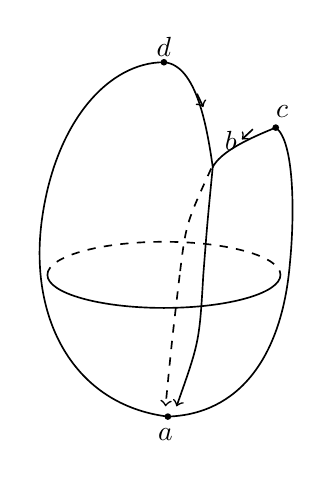
\begin{tikzpicture}[line width=0.6pt,scale=1.0]
  \draw (0.05,-2.15) .. controls (-1.15,-2.0) and (-1.72,-0.9) .. (-1.55,0.35)
        .. controls (-1.38,1.6) and (-0.7,2.35) .. (0,2.35)
        .. controls (0.42,2.32) and (0.55,1.5) .. (0.62,1.02)
        .. controls (0.72,1.2) and (1.0,1.35) .. (1.42,1.52)
        .. controls (1.66,1.35) and (1.66,0.4) .. (1.6,-0.2)
        .. controls (1.5,-1.4) and (0.95,-2.12) .. (0.05,-2.15);
  \fill (0,2.35) circle (1.2pt);
  \fill (1.42,1.52) circle (1.2pt);
  \fill (0.05,-2.15) circle (1.2pt);
  \draw[dashed] (-1.48,-0.35) arc (180:0:1.48 and 0.42);
  \draw (-1.48,-0.35) arc (180:360:1.48 and 0.42);
  \draw (0.62,1.02) .. controls (0.55,0.3) .. (0.5,-0.35);
  \draw[->] (0.5,-0.35) .. controls (0.45,-1.2) .. (0.16,-2.02);
  \draw[dashed] (0.6,1.0) .. controls (0.28,0.3) .. (0.2,-0.35);
  \draw[->,dashed] (0.2,-0.35) .. controls (0.1,-1.2) .. (0.02,-2.02);
  \draw[->] (0.42,1.95) -- (0.5,1.78);
  \draw[->] (1.13,1.5) -- (0.99,1.37);
  \node at (0,2.55) {$d$};
  \node at (1.5,1.72) {$c$};
  \node at (0.85,1.35) {$b$};
  \node at (0.02,-2.38) {$a$};
\end{tikzpicture}
\caption{“另一”\trSphere}
\label{fig:other-sphere}
\end{minipage}\hfill
\begin{minipage}[b]{0.48\textwidth}
\centering
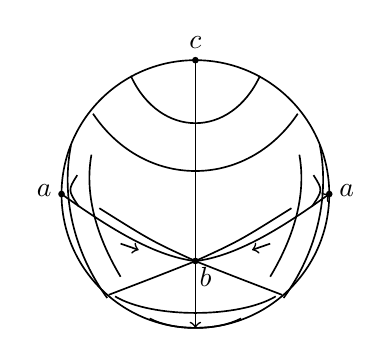
\begin{tikzpicture}[line width=0.6pt,scale=1.0]
  \draw (0,0) circle (1.7);
  \fill (0,1.7) circle (1.2pt);
  \fill (-1.7,0) circle (1.2pt);
  \fill (1.7,0) circle (1.2pt);
  \fill (0,-0.85) circle (1.2pt);
  \draw (-1.7,0) .. controls (-1.0,-0.5) and (-0.5,-0.78) .. (-0.02,-0.85);
  \draw[->] (0.02,-0.85) .. controls (0.5,-0.78) and (1.0,-0.5) .. (1.7,0);
  \draw[->] (-0.95,-0.63) -- (-0.72,-0.71);
  \draw[->] (0.95,-0.63) -- (0.72,-0.71);
  \draw (0,1.7) -- (0,-0.05);
  \draw[->] (0,-0.05) -- (0,-1.7);
  \draw (-1.1,-1.28) .. controls (-0.5,-1.05) .. (-0.02,-0.86)
        .. controls (0.55,-0.6) .. (1.22,-0.18);
  \draw (1.1,-1.28) .. controls (0.5,-1.05) .. (0.02,-0.86)
        .. controls (-0.55,-0.6) .. (-1.22,-0.18);
  \draw (-0.82,1.5) .. controls (-0.45,0.7) and (0.45,0.7) .. (0.82,1.5);
  \draw (-1.3,1.02) .. controls (-0.65,0.05) and (0.65,0.05) .. (1.3,1.02);
  \draw (-1.02,-1.3) .. controls (-0.55,-1.58) and (0.55,-1.58) .. (1.02,-1.3);
  \draw (-0.58,-1.58) .. controls (-0.28,-1.74) and (0.28,-1.74) .. (0.58,-1.58);
  \draw (-1.58,0.62) .. controls (-1.72,-0.1) and (-1.5,-0.8) .. (-1.12,-1.32);
  \draw (1.58,0.62) .. controls (1.72,-0.1) and (1.5,-0.8) .. (1.12,-1.32);
  \draw (-1.32,0.5) .. controls (-1.42,-0.05) and (-1.22,-0.6) .. (-0.95,-1.05);
  \draw (1.32,0.5) .. controls (1.42,-0.05) and (1.22,-0.6) .. (0.95,-1.05);
  \draw (-1.5,0.24) .. controls (-1.62,0.05) .. (-1.48,-0.16);
  \draw (1.5,0.24) .. controls (1.62,0.05) .. (1.48,-0.16);
  \node at (0,1.92) {$c$};
  \node at (-1.92,0.05) {$a$};
  \node at (1.92,0.05) {$a$};
  \node at (0.13,-1.05) {$b$};
\end{tikzpicture}
\caption{\trProjectivePlane}
\label{fig:projective-plane}
\end{minipage}
\end{figure}

\emph{$\CP^2(\RR)$上的\trMorseFunction。}

至于\cref{fig:projective-plane}，它展示的则是实\trProjectivePlane{} $\CP^2(\RR)$ 上那个先前（在\cref{ex:ch01-06}中）考虑过的函数的三个\trCriticalPoint{}——$a$（极小点）、$b$（\trIndex{}~1）与 $c$（极大点）——的\trStableManifold{}与\trUnstableManifold。

\subsection{\trSmaleCondition}
\label{subsec:smale-condition}

我们说，\trAdapted{}于\trMorseFunction{} $f$ 的一个\trPseudogradient{}场满足\textbf{\trSmaleCondition}（Smale condition），如果它的各\trCriticalPoint{}的\trStableManifold{}与\trUnstableManifold{}全都\trTransverse{}相交，也就是说，如果
\[
\text{对 $f$ 的所有\trCriticalPoint{} $a$、$b$，}\qquad W^u(a)\pitchfork W^s(b)\text{。}
\]

\begin{remark}\label{thm:always-transversal}
某些\trStableManifold{}与\trUnstableManifold{}总是\trTransverse{}相交的。例如，我们总有：
\begin{itemize}
\item $W^u(a)\pitchfork W^s(a)$（对同一个\trCriticalPoint{}而言），这正是我们在 $a$ 附近的一张\trMorseChart{}中所看到的情形；
\item 若 $a$ 与 $b$ 不同且 $f(a)\le f(b)$，则 $W^u(a)\cap W^s(b)=\varnothing$（特别地，这些\trStableManifold{}与\trUnstableManifold{}是\trTransverse{}的）。
\end{itemize}
如果这个\trVectorField{}满足\trSmaleCondition，那么对\trCriticalPoint{} $a$ 与 $b$ 的每一种组合都有
\[
\operatorname{codim}\bigl(W^u(a)\cap W^s(b)\bigr)=\operatorname{codim}\, W^u(a)+\operatorname{codim}\, W^s(b)\text{，}
\]
也就是说
\[
\dim\bigl(W^u(a)\cap W^s(b)\bigr)=\operatorname{Ind}(a)-\operatorname{Ind}(b)\text{。}
\]
在我们的条件之下，这个交是 $V$ 的一个\trSubmanifold，我们把它记作 $\mathcal{M}(a,b)$。它由连接 $a$ 与 $b$ 的那些\trTrajectory{}上的全部点构成：
\[
\mathcal{M}(a,b)=\Bigl\{x\in V \Bigm| \lim_{s\to-\infty}\varphi^s(x)=a\ \text{且}\ \lim_{s\to+\infty}\varphi^s(x)=b\Bigr\}\text{。}
\]
\end{remark}

\begin{proposition}\label{thm:translation-action-free}
时间平移群 $\RR$ 作用在 $\mathcal{M}(a,b)$ 上，作用方式为 $s\cdot x=\varphi^s(x)$。当 $a\neq b$ 时，这个作用是自由的。
\end{proposition}

\begin{proof}
这显然构成一个群作用。设 $a\neq b$，此时 $\mathcal{M}(a,b)$ 中没有\trCriticalPoint。任取 $x\in\mathcal{M}(a,b)$。由于 $x$ 不是\trCriticalPoint，我们知道 $f(\varphi^s(x))$ 是 $s$ 的递减函数，因此若 $\varphi^s(x)=\varphi^{s'}(x)$，则必有 $s=s'$。所以这个作用是自由的。
\end{proof}

于是，这个商是一个\trManifold，我们把它记作 $\mathcal{L}(a,b)$。它的维数为
\[
\dim\mathcal{L}(a,b)=\operatorname{Ind}(a)-\operatorname{Ind}(b)-1\text{。}
\]

\begin{remark}\label{thm:quotient-level-set}
十分清楚，这个商是一个分离的空间。实际上，考虑这个商最为方便的方式如下。设 $\alpha$ 是介于 $f(a)$ 与 $f(b)$ 之间的 $f$ 的一个值，那么 $\mathcal{M}(a,b)$ 与\trLevelSet{} $f^{-1}(\alpha)$ \trTransverse{}相交：这张\trLevelSet{}的余维数为~1，而\trVectorField{} $X$ 与它\trTransverse{}（按定义，$X$ 不会切于这张\trLevelSet，否则就要在一个非\trCriticalPoint{}处有 $df(X)=0$）。从 $a$ 出发的诸\trTrajectory{}都恰好在这张中间\trLevelSet{}上经过一点，因此可以把 $\mathcal{L}(a,b)$ 与 $\mathcal{M}(a,b)\cap f^{-1}(\alpha)$ 等同起来。
\end{remark}

于是，设 $a$ 与 $b$ 是两个（不同的）\trCriticalPoint，若所用的\trGradient{}满足\trSmaleCondition，那么要想 $\mathcal{M}(a,b)$ 或 $\mathcal{L}(a,b)$ 非空，就必须
\[
\operatorname{Ind}(a)>\operatorname{Ind}(b)\text{。}
\]
换句话说，\trIndex{}沿着诸条\trGradient{}线递减。

在下一章里，我们将回过头来详细讨论这些空间。

\begin{example}\label{thm:examples-smale-condition}
上面给出的所有例子都满足\trSmaleCondition\footnote{在“另一”\trSphere{}与\trProjectivePlane{}的情形，例如可以借助\cref{ex:ch02-11}来验证这一点。}，惟\trTorus{}上的\trHeightFunction{}一例除外。事实上，$W^s(b)$ 与 $W^u(c)$ 并不\trTransverse——这一点我们在\cref{subsec:examples-stable-unstable}与\cref{fig:height-torus}的例子中其实早已注意到，只是未曾自觉罢了。此外，这里还有连接两个\trIndex{}为~1 的\trCriticalPoint{}的\trTrajectory，而我们方才已经看到，这是被禁止的。这个“坏”的\trVectorField，就是\trTorus{}上由外围\trEuclidean{}\trMetric{}所诱导的\trRiemann{}\trMetric{}下的那个\trGradient。
\end{example}

\trSmaleCondition{}禁止\cref{fig:bad-flow}那类\trFlowLine{}的存在。\cref{fig:perturbed-flow}画的则是一个满足\trSmaleCondition{}的邻近场的诸\trTrajectory（它由下一小节所解释的一般方法求得）。

\begin{figure}[htbp]
\begin{minipage}[b]{0.48\textwidth}
\centering
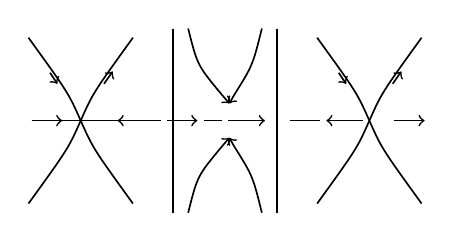
\begin{tikzpicture}[line width=0.6pt,scale=0.78]
  \draw (-0.85,1.35) .. controls (-0.2,0.45) .. (0,0) .. controls (0.2,-0.45) .. (0.85,-1.35);
  \draw[->] (-0.5,0.78) -- (-0.38,0.6);
  \draw (-0.85,-1.35) .. controls (-0.2,-0.45) .. (0,0) .. controls (0.2,0.45) .. (0.85,1.35);
  \draw[->] (0.38,0.6) -- (0.52,0.8);
  \draw[shift={(4.7,0)}] (-0.85,1.35) .. controls (-0.2,0.45) .. (0,0) .. controls (0.2,-0.45) .. (0.85,-1.35);
  \draw[->] (4.2,0.78) -- (4.32,0.6);
  \draw[shift={(4.7,0)}] (-0.85,-1.35) .. controls (-0.2,-0.45) .. (0,0) .. controls (0.2,0.45) .. (0.85,1.35);
  \draw[->] (5.08,0.6) -- (5.22,0.8);
  \draw (1.5,1.5) -- (1.5,-1.5);
  \draw (3.2,1.5) -- (3.2,-1.5);
  \draw (-0.8,0) -- (1.2,0); \draw[->] (-0.8,0) -- (-0.3,0);
  \draw[->] (1.3,0) -- (0.6,0); \draw[->] (1.4,0) -- (1.9,0); \draw (2.0,0) -- (2.3,0);
  \draw[->] (2.4,0) -- (3.0,0); \draw (3.4,0) -- (3.9,0);
  \draw[->] (4.6,0) -- (4.0,0);
  \draw[->] (5.1,0) -- (5.6,0);
  \draw (1.75,1.5) .. controls (1.9,0.9) .. (2.3,0.42);
  \draw[->] (2.3,0.42) -- (2.42,0.28);
  \draw (2.95,1.5) .. controls (2.8,0.9) .. (2.5,0.42);
  \draw[->] (2.5,0.42) -- (2.42,0.28);
  \draw (1.75,-1.5) .. controls (1.9,-0.9) .. (2.3,-0.42);
  \draw[->] (2.3,-0.42) -- (2.42,-0.28);
  \draw (2.95,-1.5) .. controls (2.8,-0.9) .. (2.5,-0.42);
  \draw[->] (2.5,-0.42) -- (2.42,-0.28);
\end{tikzpicture}
\caption{}
\label{fig:bad-flow}
\end{minipage}\hfill
\begin{minipage}[b]{0.48\textwidth}
\centering
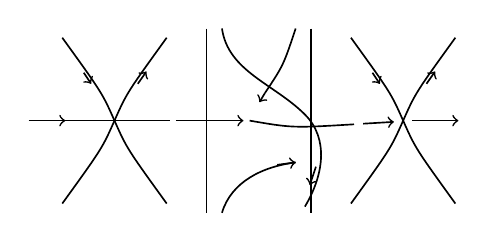
\begin{tikzpicture}[line width=0.6pt,scale=0.78]
  \draw (-0.85,1.35) .. controls (-0.2,0.45) .. (0,0) .. controls (0.2,-0.45) .. (0.85,-1.35);
  \draw[->] (-0.5,0.78) -- (-0.38,0.6);
  \draw (-0.85,-1.35) .. controls (-0.2,-0.45) .. (0,0) .. controls (0.2,0.45) .. (0.85,1.35);
  \draw[->] (0.38,0.6) -- (0.52,0.8);
  \draw[shift={(4.7,0)}] (-0.85,1.35) .. controls (-0.2,0.45) .. (0,0) .. controls (0.2,-0.45) .. (0.85,-1.35);
  \draw[->] (4.2,0.78) -- (4.32,0.6);
  \draw[shift={(4.7,0)}] (-0.85,-1.35) .. controls (-0.2,-0.45) .. (0,0) .. controls (0.2,0.45) .. (0.85,1.35);
  \draw[->] (5.08,0.6) -- (5.22,0.8);
  \draw (1.5,1.5) -- (1.5,-1.5);
  \draw (3.2,1.5) -- (3.2,-1.5);
  \draw[->] (-1.4,0) -- (-0.8,0);
  \draw (-1.2,0) -- (0.9,0); \draw[->] (1.0,0) -- (2.1,0);
  \draw (2.2,0) .. controls (2.9,-0.12) .. (3.9,-0.06);
  \draw[->] (4.05,-0.05) -- (4.55,-0.02);
  \draw (4.85,0) -- (5.6,0); \draw[->] (5.0,0) -- (5.6,0);
  \draw (1.75,1.5) .. controls (1.85,0.8) and (2.6,0.6) .. (3.1,0.1)
        .. controls (3.5,-0.3) and (3.4,-0.9) .. (3.1,-1.4);
  \draw[->] (3.28,-0.75) -- (3.18,-1.05);
  \draw (2.95,1.5) .. controls (2.75,0.9) .. (2.45,0.45);
  \draw[->] (2.45,0.45) -- (2.36,0.3);
  \draw (1.75,-1.5) .. controls (1.9,-1.0) and (2.4,-0.75) .. (2.95,-0.68);
  \draw[->] (2.65,-0.72) -- (2.95,-0.68);
\end{tikzpicture}
\caption{}
\label{fig:perturbed-flow}
\end{minipage}
\end{figure}

\subsection{存在性}
\label{subsec:existence}

现在，让我们沿用 [72] 来证明：满足\trSmaleCondition{}的\trPseudogradient{}场是存在的，而且是\trGeneric{}的。

我们首先注意：必要时，只需把 $f$ 换成另一个在 $\cC^1$ 意义下任意接近的函数，便可以——而且我们也确实要——假定 $f$ 在它的所有\trCriticalPoint{}处取互不相同的值。事实上，在 $\Omega$ 之外，由\trCompact{}性可知，对某个 $\varepsilon_0>0$ 有 $df(X)<-\varepsilon_0$。于是我们选取一个在每张\trMorseChart{} $\Omega_i$ 上都取常值、满足 $|dh|<\frac{1}{2}\varepsilon_0$、并且使得
\[
f(c_i)+h(c_i)\neq f(c_j)+h(c_j)\qquad\text{对 } i\neq j
\]
的函数 $h$。函数 $f+h$ 仍是\trMorseFunction，其\trCriticalPoint{}与 $f$ 的相同，\trVectorField{} $X$ 也仍是一个\trAdapted{}的\trPseudogradient，只是诸\trCriticalValue{}现在互不相同了。

\begin{theorem}[\trSmale{}定理~{[72]}]\label{thm:smale-theorem}\BookIndexDefinition{T010}
设 $V$ 是一个\trManifoldWithBoundary，并设 $f$ 是 $V$ 上诸\trCriticalValue{}互不相同的一个\trMorseFunction。我们在 $f$ 的每个\trCriticalPoint{}的邻域内取定\trMorseChart。设 $\Omega$ 为这些\trChart{}的并集，并设 $X$ 是 $V$ 上一个\trTransverse{}于边界的\trPseudogradient{}场。那么，存在一个\trPseudogradient{}场 $X'$，它在 $\cC^1$ 意义下邻近于 $X$、在 $\Omega$ 上等于 $X$，并且对 $f$ 的所有\trCriticalPoint{} $a$、$b$ 都有
\[
W^s_{X'}(a)\pitchfork W^u_{X'}(b)\text{。}
\]
\end{theorem}

我们来澄清这里所用的 $\cC^1$ 意义下的\textbf{邻近}（proximity）概念：这条陈述断言，对每个 $\varepsilon>0$、对 $V$ 的每一个由\trChart{} $\varphi_i(U_i)$ 构成的\trCovering、以及对每个\trCompact{}子集 $K_i\subset U_i$，都存在一个\trVectorField{} $X'$，使得
\[
\bigl\|T\varphi_i^{-1}(X')-T\varphi_i^{-1}(X)\bigr\|<\varepsilon
\]
在 $K_i$ 上关于 $\cC^1$ 范数成立，并且前述诸性质也成立。

\begin{remark}\label{thm:good-approximation}
一个在 $\cC^1$ 意义下充分接近\trPseudogradient{}场 $X$、并且在 $\Omega$ 上等于 $X$ 的\trVectorField{} $X'$，本身就是一个\trPseudogradient{}场。为简便起见，我们将把这样的 $X'$ 称为 $X$ 的一个“好逼近”（good approximation）。
\end{remark}

\begin{remark}\label{thm:kupka-smale}\BookIndexDefinition{T011}
这条定理有时称作“库普卡--\trSmale”定理，因为 库普卡 也给出过一个证明。我们此处模仿的是\trSmale{}的证明。
\end{remark}

\begin{proof}[\cref{thm:smale-theorem}的证明]
由于 $f$ 的诸\trCriticalValue{}互不相同，把它们按大小排列为
\[
\operatorname{Crit}(f)=\{c_1,\dotsc,c_q\}\text{，}\qquad f(c_1)>f(c_2)>\dotsb>f(c_q)\text{，}
\]
并令 $\alpha_i=f(c_i)$。定理的证明将使用一种基于下述引理的归纳法。

\begin{lemma}\label{thm:stable-transversal-approx}
设 $j\in\{1,\dotsc,q\}$，并设 $\varepsilon>0$ 充分小（使 $\alpha_j+2\varepsilon<\alpha_{j-1}$；$j=1$ 情形平凡）。\footnote{译注：原书此处仅设 $\varepsilon>0$；然当 $\varepsilon>\max f-\alpha_j$ 时 $f^{-1}([\alpha_j+\varepsilon,\alpha_j+2\varepsilon])=\varnothing$，条件 (1) 遂要求 $X'$ 在整个 $V$ 上与 $X$ 重合，而一般的 $X$ 未必满足条 (2)（其证明开篇即改取充分小的 $\varepsilon$ 使 $\alpha_j+2\varepsilon<\alpha_{j-1}$，可见陈述疑漏“充分小”之限定）；此处径改。——译者注}那么存在 $X$ 的一个（$\cC^1$ 意义下的）好逼近 $X'$，使得：
\begin{enumerate}[label=(\arabic*)]
\item \trVectorField{} $X'$ 在 $V$ 中 $f^{-1}\bigl([\alpha_j+\varepsilon,\alpha_j+2\varepsilon]\bigr)$ 的补集上与 $X$ 相重合；
\item $c_j$ 的\trStableManifold{}（对 $X'$ 而言）与所有\trCriticalPoint{}的\trUnstableManifold{}\trTransverse{}相交，也就是说，
\[
W^s_{X'}(c_j)\pitchfork W^u_{X'}(c_i)\text{。}
\]
\end{enumerate}
\end{lemma}

让我们暂且承认这条引理，来证明定理。令 $\scr{P}(r)$ 表示下述性质：存在 $X$ 的一个好逼近 $X'_r$，使得对每个 $p\le r$ 及每个 $i$，都有
\[
W^s_{X'_r}(c_p)\pitchfork W^u_{X'_r}(c_i)\text{。}
\]

注意：
\begin{itemize}
\item 性质 $\scr{P}(q)$ 恰好就是定理本身。
\item 性质 $\scr{P}(1)$ 成立的理由是平凡的：\trCriticalPoint{} $c_1$ 是 $f$ 的极大点，其\trStableManifold{}缩成它自身，因而它不与任何位于 $c_1$ 之下的\trCriticalPoint{}的\trUnstableManifold{}相交。
\item 而性质 $\scr{P}(2)$ 则由 $j=2$ 时的引理得到。
\end{itemize}

于是，让我们假定 $\scr{P}(r-1)$ 为真，来证明 $\scr{P}(r)$ 也为真。我们有一个\trVectorField{} $X'_{r-1}$，使得 $c_{r-1}$ 的\trStableManifold{}与所有\trUnstableManifold{}\trTransverse。把引理应用到\trVectorField{} $X'_{r-1}$ 与 $j=r$。这给出一个\trVectorField{} $X'_r$，它（这是引理给出的第一条性质）特别地在 $\alpha_r+\varepsilon\le f\le\alpha_r+2\varepsilon$ 这条窄带之外与 $X'_{r-1}$ 相重合。此外，由于对每个 $p\le r-1$ 而言，$X'_{r-1}$ 之下 $c_p$ 的\trStableManifold{}都位于这条窄带的上方，故该\trStableManifold{}对 $X'_{r-1}$ 而言与对 $X'_r$ 而言是同一个（参见\cref{fig:strip}）。于是我们有
\[
W^s_{X'_{r-1}}(c_p)\cap W^u_{X'_{r-1}}(c_i)=W^s_{X'_r}(c_p)\cap W^u_{X'_r}(c_i)
\]
对 $p\le r-1$ 及每个 $i$ 成立，从而
\[
W^s_{X'_r}(c_p)\pitchfork W^u_{X'_r}(c_i)\text{。}
\]
对 $p=r$，引理蕴含（这是第二条性质）：
\[
W^s_{X'_r}(c_r)\pitchfork W^u_{X'_r}(c_i)\text{。}\qedhere
\]
\end{proof}

\begin{figure}[htbp]
\centering
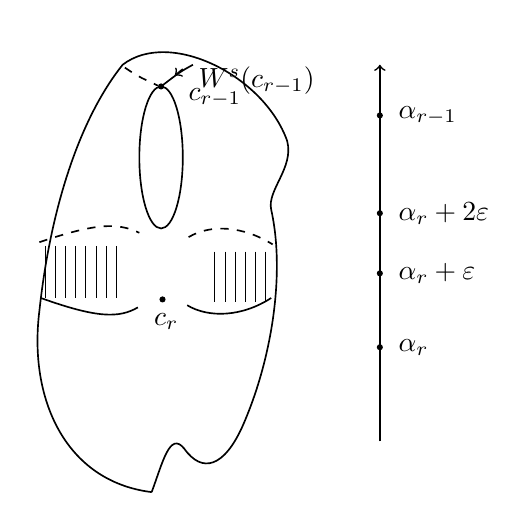
\begin{tikzpicture}[line width=0.6pt,scale=0.92]
  \draw (-0.15,-3.3) .. controls (-1.35,-3.15) and (-1.85,-2.0) .. (-1.7,-0.8)
        .. controls (-1.55,0.6) and (-1.15,1.85) .. (-0.55,2.60)
        .. controls (0.10,3.10) and (1.40,2.45) .. (1.72,1.55)
        .. controls (1.82,1.18) and (1.44,0.87) .. (1.5,0.6)
        .. controls (1.7,-0.3) and (1.5,-1.5) .. (1.1,-2.4)
        .. controls (0.85,-2.95) and (0.55,-3.05) .. (0.3,-2.7)
        .. controls (0.1,-2.45) and (-0.0,-2.9) .. (-0.15,-3.3);
  \foreach \x in {-1.62,-1.48,-1.34,-1.20,-1.06,-0.92,-0.78,-0.64}{
    \draw[very thin] (\x,0.1) -- (\x,-0.62);
  }
  \foreach \x in {0.72,0.86,1.00,1.14,1.28,1.42}{
    \draw[very thin] (\x,0.02) -- (\x,-0.68);
  }
  \draw[dashed] (-1.7,0.15) .. controls (-0.9,0.42) and (-0.62,0.42) .. (-0.32,0.28);
  \draw[dashed] (0.36,0.22) .. controls (0.66,0.4) and (1.1,0.38) .. (1.52,0.12);
  \draw (-1.68,-0.62) .. controls (-0.9,-0.9) and (-0.6,-0.9) .. (-0.34,-0.75);
  \draw (0.34,-0.72) .. controls (0.64,-0.9) and (1.1,-0.88) .. (1.5,-0.62);
  \draw (-0.02,1.32) ellipse (0.30 and 0.98);
  \fill (-0.02,2.3) circle (1.2pt);
  \fill (0.0,-0.64) circle (1.2pt);
  \draw[dashed] (-0.52,2.56) .. controls (-0.34,2.44) .. (-0.06,2.31);
  \draw (0.42,2.6) .. controls (0.24,2.5) .. (-0.02,2.3);
  \draw[->] (0.28,2.54) -- (0.17,2.45);
  \draw[->] (3.0,-2.6) -- (3.0,2.6);
  \fill (3.0,1.9) circle (1.2pt);
  \node[right] at (3.12,1.9) {$\alpha_{r-1}$};
  \fill (3.0,0.55) circle (1.2pt);
  \node[right] at (3.12,0.55) {$\alpha_r+2\varepsilon$};
  \fill (3.0,-0.28) circle (1.2pt);
  \node[right] at (3.12,-0.28) {$\alpha_r+\varepsilon$};
  \fill (3.0,-1.3) circle (1.2pt);
  \node[right] at (3.12,-1.3) {$\alpha_r$};
  \node[right] at (0.36,2.38) {$W^s(c_{r-1})$};
  \node[right] at (0.22,2.14) {$c_{r-1}$};
  \node[below] at (0.05,-0.7) {$c_r$};
\end{tikzpicture}
\caption{}
\label{fig:strip}
\end{figure}

\begin{proof}[\cref{thm:stable-transversal-approx}的证明]
考虑 $c_j$ 邻域内的一张\trMorseChart{}可能是有用的。\cref{fig:morse-chart-level}把它画了出来（画了两次）。我们选取充分小的 $\varepsilon$，使得
\[
\alpha_j+2\varepsilon<\alpha_{j-1}\text{。}
\]
设 $k$ 为 $c_j$ 的\trIndex，并令 $Q=W^s(c_j)\cap f^{-1}(\alpha_j+2\varepsilon)$。那么 $Q$ 是一个维数为 $n-k-1$ 的\trSphere。我们考虑这张\trSphere{} $Q$ 在 $f^{-1}(\alpha_j+2\varepsilon)$ 内的一个\textbf{\trTubularNeighborhood}（tubular neighborhood），其形状为 $Q\times D^k$；我们在\cref{fig:morse-chart-level}中的一张\trMorseChart{}里、以及在\cref{fig:in-the-manifold}中都可以看到它。

\begin{figure}[htbp]
\centering
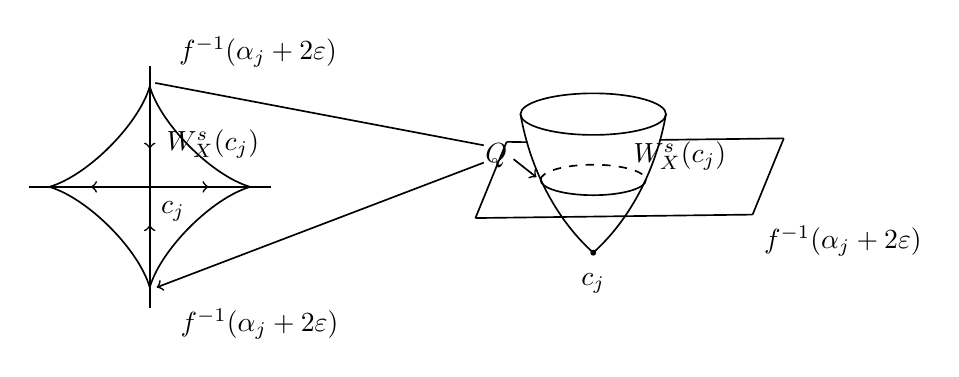
\begin{tikzpicture}[line width=0.6pt,scale=0.88]
  \begin{scope}[xshift=0cm]
    \draw (0,1.45) .. controls (0.16,0.9) and (0.9,0.16) .. (1.45,0)
          .. controls (0.9,-0.16) and (0.16,-0.9) .. (0,-1.45)
          .. controls (-0.16,-0.9) and (-0.9,-0.16) .. (-1.45,0)
          .. controls (-0.9,0.16) and (-0.16,0.9) .. (0,1.45);
    \draw (0,-1.75) -- (0,1.75);
    \draw (-1.75,0) -- (1.75,0);
    \draw[->] (0,0.85) -- (0,0.55);
    \draw[->] (0,-0.85) -- (0,-0.55);
    \draw[->] (-0.55,0) -- (-0.85,0);
    \draw[->] (0.55,0) -- (0.85,0);
    \node[right] at (0.1,0.62) {$W^s_X(c_j)$};
    \node[below right] at (0.02,-0.06) {$c_j$};
    \node[above right] at (0.28,1.58) {$f^{-1}(\alpha_j+2\varepsilon)$};
    \node[below right] at (0.3,-1.62) {$f^{-1}(\alpha_j+2\varepsilon)$};
  \end{scope}
  \begin{scope}[xshift=6.4cm]
    \draw (-1.25,0.65) -- (-0.95,0.645);
    \draw (0.96,0.678) -- (2.75,0.70);
    \draw (-1.7,-0.45) -- (-1.25,0.65);
    \draw (2.3,-0.40) -- (2.75,0.70);
    \draw (-1.7,-0.45) -- (2.3,-0.40);
    \draw (0,1.05) ellipse (1.05 and 0.3);
    \draw (-1.05,1.05) .. controls (-0.9,0.2) and (-0.5,-0.5) .. (0,-0.95);
    \draw (1.05,1.05) .. controls (0.9,0.2) and (0.5,-0.5) .. (0,-0.95);
    \draw[dashed] (-0.76,0.10) arc (180:0:0.76 and 0.22);
    \draw (-0.76,0.10) arc (180:360:0.76 and 0.22);
    \node at (1.25,0.45) {$W^s_X(c_j)$};
    \fill (0,-0.95) circle (1.2pt);
    \node[below] at (0,-1.1) {$c_j$};
    \node[below right] at (2.32,-0.42) {$f^{-1}(\alpha_j+2\varepsilon)$};
  \end{scope}
  \node at (5.0,0.45) {$Q$};
  \draw (4.82,0.6) -- (0.08,1.5);
  \draw[->] (4.82,0.35) -- (0.1,-1.45);
  \draw[->] (5.25,0.4) -- (5.58,0.14);
\end{tikzpicture}
\caption{在一张\trMorseChart{}中}
\label{fig:morse-chart-level}
\end{figure}

于是，存在一个\trEmbedding\footnote{译注：原书此处以 $]a,b[$ 记开区间，即通常记法的 $(a,b)$。}
\[
\boldsymbol{\Psi}\colon D^k\times Q\times[0,m]\longrightarrow f^{-1}\bigl(\,]\alpha_j+\varepsilon,\,\alpha_j+2\varepsilon[\,\bigr)
\]
使得：
\begin{itemize}
\item $\boldsymbol{\Psi}$ 限制在 $\{0\}\times Q\times\{0\}$ 上，正是 $Q$ 在 $f^{-1}(\alpha_j+\varepsilon)$ 中的那个\trEmbedding；\footnote{译注：$z=0$ 与 $z=m$ 两端的像落在闭带 $f^{-1}\bigl(\,[\alpha_j+\varepsilon,\,\alpha_j+2\varepsilon]\,\bigr)$ 的两端面上，而所示目标开带 $f^{-1}\bigl(\,]\alpha_j+\varepsilon,\,\alpha_j+2\varepsilon[\,\bigr)$ 不含这两面；按其用法宜写作闭带（内部为\trEmbedding、端面为延拓）。此处照原书排印，存疑备案。——译者注}
\item $\boldsymbol{\Psi}$ 限制在 $\{0\}\times Q\times\{m\}$ 上，正是 $Q$ 在 $f^{-1}(\alpha_j+2\varepsilon)$ 中的那个\trEmbedding；
\item 若 $z$ 是 $[0,m]\subset\RR$ 中的坐标，则
\[
\boldsymbol{\Psi}_*\Bigl(-\frac{\partial}{\partial z}\Bigr)=X\text{。}
\]
\end{itemize}

诸\trUnstableManifold{}与诸\trLevelSet{}\trTransverse{}相交。特别地，它们沿着一个（一般并不\trConnected{}的）\trManifold{} $P'$ 与 $D^k\times Q$ 相交。若 $W^s_X(c_j)\pitchfork P'$，则无可再证。因此，证明就在于把 $X$ 在 $f^{-1}\bigl(\,]\alpha_j+\varepsilon,\,\alpha_j+2\varepsilon[\,\bigr)$ 上修改成 $X'$，使得
\[
W^s_{X'}(c_j)\pitchfork P'\text{。}
\]

这一修改将在 $\boldsymbol{\Psi}$ 的像内进行。于是，让我们置身于 $D^k\times Q\times[0,m]$ 之中并取 $X=-\partial/\partial z$。\cref{fig:in-the-manifold}画的是\trManifold{}中发生的事情，而\cref{fig:model}画的则是模型。

\begin{figure}[htbp]
\centering
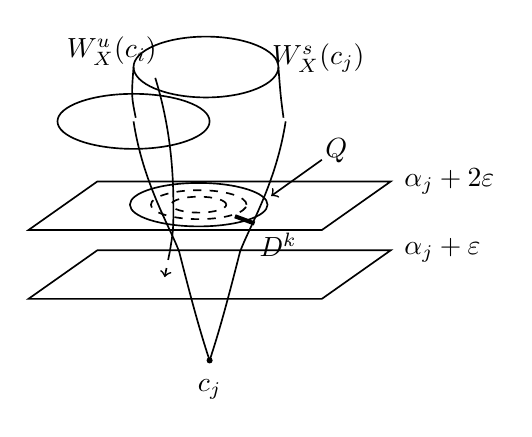
\begin{tikzpicture}[line width=0.6pt,scale=0.92]
  \draw (-2.5,0.25) -- (1.55,0.25) -- (2.5,0.92) -- (-1.55,0.92) -- cycle;
  \draw (-2.5,-0.7) -- (1.55,-0.7) -- (2.5,-0.03) -- (-1.55,-0.03) -- cycle;
  \node[right] at (2.55,0.92) {$\alpha_j+2\varepsilon$};
  \node[right] at (2.55,-0.03) {$\alpha_j+\varepsilon$};
  \draw (-1.05,1.75) ellipse (1.05 and 0.38);
  \draw (-1.05,1.75) .. controls (-0.92,0.9) and (-0.55,0.3) .. (-0.42,-0.05)
        .. controls (-0.28,-0.6) and (-0.15,-1.1) .. (0,-1.55);
  \draw (1.05,1.75) .. controls (0.92,0.9) and (0.55,0.3) .. (0.42,-0.05)
        .. controls (0.28,-0.6) and (0.15,-1.1) .. (0,-1.55);
  \fill (0,-1.55) circle (1.2pt);
  \node[below] at (0,-1.68) {$c_j$};
  \draw (-0.15,0.6) ellipse (0.95 and 0.3);
  \draw[dashed] (-0.15,0.6) ellipse (0.66 and 0.2);
  \draw[dashed] (-0.15,0.6) ellipse (0.38 and 0.11);
  \draw (-0.05,2.5) ellipse (1.0 and 0.42);
  \draw (-1.05,2.5) .. controls (-1.08,2.1) .. (-1.02,1.8);
  \draw (0.95,2.5) .. controls (0.98,2.1) .. (1.02,1.8);
  \draw (-0.75,2.35) .. controls (-0.55,1.7) and (-0.5,1.1) .. (-0.5,0.6)
        .. controls (-0.5,0.25) .. (-0.55,-0.05);
  \draw[->,dashed] (-0.55,-0.05) -- (-0.62,-0.4);
  \node at (-1.35,2.72) {$W^u_X(c_i)$};
  \node at (1.5,2.62) {$W^s_X(c_j)$};
  \node at (1.75,1.35) {$Q$};
  \draw[->] (1.55,1.22) -- (0.85,0.72);
  \draw[line width=1.5pt] (0.35,0.44) -- (0.62,0.34);
  \node[below right] at (0.55,0.35) {$D^k$};
\end{tikzpicture}
\caption{在\trManifold{}中}
\label{fig:in-the-manifold}
\end{figure}

设 $P$ 为\trSubmanifold{} $\boldsymbol{\Psi}^{-1}(P')\subset D^k\times Q\times[0,m]$。正如在模型中所见，我们所要的\trTransversality{}条件 $W^s_{X'}(c_j)\pitchfork P'$ 可以写成
\[
W^s_{X'}\pitchfork P\qquad\text{其中}\quad W^s_{X'}=\bigl\{\varphi^{-s}_{X'}(0,q,0)\ \bigm|\ s>0,\ q\in Q\bigr\}\text{。}
\]

在初始情形，$X'=X=-\partial/\partial z$，于是
\[
P\cap W^s_X=P\cap\{(0,q,s)\mid s>0,\ q\in Q\}=P\cap\{(0,q,0)\mid q\in Q\}=g^{-1}(0)\text{，}
\]
其中 $g\colon P\to D^k$ 是投影 $(x,q,z)\mapsto x$。\footnote{译注：原书此链式等式中间项印作 $P\cap\{(0,q,0)\mid q\in Q\}$；与前一集 $\{s>0\}$ 不相衔接，疑为 $P\cap(\{0\}\times Q\times[0,m])$ 之误；此处照原书排印，存疑备案。——译者注}

\begin{figure}[htbp]
\centering
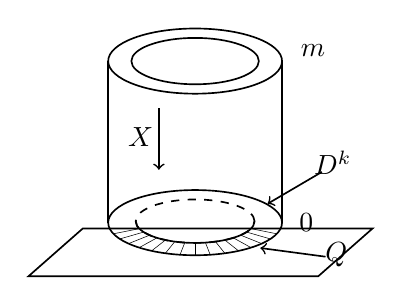
\begin{tikzpicture}[line width=0.6pt,scale=0.92]
  \draw (-2.3,-0.72) -- (1.7,-0.72) -- (2.45,-0.06) -- (-1.55,-0.06) -- cycle;
  \draw (0,0.02) ellipse (1.2 and 0.45);
  \draw[dashed] (0,0.04) ellipse (0.82 and 0.3);
  \draw (-0.82,0.04) arc (180:360:0.82 and 0.3);
  \foreach \a in {200,210,220,230,240,250,260,270,280,290,300,310,320,330,340}{
    \draw[very thin] ({1.2*cos(\a)},{0.02+0.45*sin(\a)}) -- ({0.82*cos(\a)},{0.04+0.3*sin(\a)});
  }
  \draw (-1.2,0.02) -- (-1.2,2.25);
  \draw (1.2,0.02) -- (1.2,2.25);
  \draw (0,2.25) ellipse (1.2 and 0.45);
  \draw (0,2.25) ellipse (0.88 and 0.32);
  \draw[->] (-0.5,1.6) -- (-0.5,0.75);
  \node at (-0.75,1.2) {$X$};
  \node[right] at (1.32,2.4) {$m$};
  \node[right] at (1.3,0.02) {$0$};
  \node at (1.9,0.85) {$D^k$};
  \draw[->] (1.75,0.72) -- (1.0,0.28);
  \node at (1.95,-0.42) {$Q$};
  \draw[->] (1.8,-0.45) -- (0.9,-0.33);
\end{tikzpicture}
\caption{模型}
\label{fig:model}
\end{figure}

证明将在于使 $0$ 成为 $g$ 的一个\trRegularValue。由\trSardTheorem，存在一个向量 $w\in D^k$，它可以任意接近 $0$（比如说 $\|w\|=\delta$），使得 $w$ 是 $g$ 的一个\trRegularValue。我们准备构造\trVectorField{} $X$ 的一个\textbf{\trPerturbation}（perturbation）$X'$，使得
\[
W^s_{X'}\cap\{z=m\}=\varphi^{-m}_{X'}(0,q,0)=(w,q,m)\text{。}
\]
那时我们将有 $W^s_{X'}\cap P=g^{-1}(w)$，这就意味着 $W^s_{X'}\cap P$ 是 $P$ 中余维数为~$k$ 的一个\trSubmanifold。等式
\[
\operatorname{codim}_P\bigl(W^s_{X'}\cap P\bigr)=\operatorname{codim}_V\, W^s_{X'}
\]
蕴含\trSubmanifold{} $W^s_{X'}$ 与 $P$ 的\trTransversality。\footnote{译注：原书此处印作 $\operatorname{codim}_P W^s_{X'}\cap P$（$\operatorname{codim}$ 后无括号）；为明确余维数所指的对象，疑应加括号；此处径加括号。——译者注}

“\trManifold{}中”的引理现在就化为下述“模型中”的引理。

\begin{lemma}\label{thm:model-vector-field}
存在一个（在 $\cC^1$ 意义下）接近 $-\partial/\partial z$ 的\trVectorField{} $X'$，使得：
\begin{enumerate}[label=(\arabic*)]
\item 在 $\partial(D^k\times Q\times[0,m])$ 附近，$X'=-\partial/\partial z$；
\item $\varphi^{-m}_{X'}(0,q,0)=(w,q,m)$。
\end{enumerate}
\end{lemma}

\begin{proof}
设 $(v_1,\dotsc,v_k)$ 是 $w\in D^k$ 的坐标。我们令
\[
X'=-\frac{\partial}{\partial z}-\sum_{i=1}^{k}\beta_i(z)\,\gamma(x)\,\frac{\partial}{\partial x_i}\text{，}
\]
其中：
\begin{itemize}
\item 函数 $\beta_i$ 在 $[0,m]$ 之外为零，满足 $|\beta_i(s)|<\eta$、$|\beta_i'(s)|<\eta$，并且 $\int_0^m\beta_i(t)\,dt=v_i$（其中 $\eta$ 是一个小的固定正数，对应于逼近所要达到的精度）；
\item 函数 $\gamma$ 则定义在 $D^k$ 上、取值于 $[0,1]$，在 $\partial D^k$ 附近恒为零，在 $\|x\|\le 1/3$ 上恒等于 $1$，并且各偏导数在 $D^k$ 上满足 $|\partial\gamma/\partial x_i|\le 2$。
\end{itemize}
参见\cref{fig:function-beta}与\cref{fig:function-gamma}。

\begin{figure}[htbp]
\begin{minipage}[b]{0.52\textwidth}
\centering
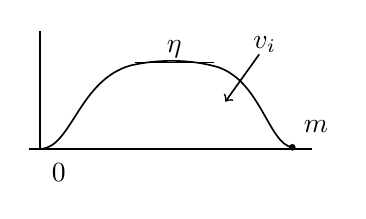
\begin{tikzpicture}[line width=0.6pt,scale=1.0]
  \draw (-0.15,0) -- (3.45,0);
  \draw (0,0) -- (0,1.5);
  \draw (0.02,0) .. controls (0.4,0.04) and (0.5,0.88) .. (1.15,1.06)
        .. controls (1.5,1.14) and (1.9,1.14) .. (2.25,1.04)
        .. controls (2.8,0.86) and (2.9,0.06) .. (3.2,0.02);
  \draw[very thin] (1.2,1.1) -- (2.2,1.1);
  \node at (1.7,1.26) {$\eta$};
  \fill (3.2,0.02) circle (1.2pt);
  \node[above right] at (3.22,0.08) {$m$};
  \node[below right] at (0.02,-0.06) {$0$};
  \node at (2.85,1.32) {$v_i$};
  \draw[->] (2.78,1.2) -- (2.35,0.6);
\end{tikzpicture}
\caption{函数 $\beta_i$}
\label{fig:function-beta}
\end{minipage}\hfill
\begin{minipage}[b]{0.42\textwidth}
\centering
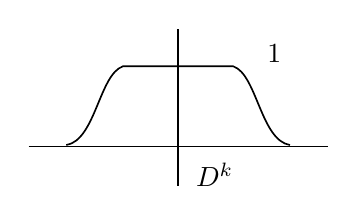
\begin{tikzpicture}[line width=0.6pt,scale=1.0]
  \draw (-1.9,0) -- (1.9,0);
  \draw (0,-0.5) -- (0,1.5);
  \draw (-1.42,0.02) .. controls (-1.05,0.08) and (-1.0,0.92) .. (-0.7,1.02)
        -- (0.7,1.02) .. controls (1.0,0.92) and (1.05,0.08) .. (1.42,0.02);
  \node at (1.22,1.18) {$1$};
  \node[below right] at (0.1,-0.08) {$D^k$};
\end{tikzpicture}
\caption{函数 $\gamma$}
\label{fig:function-gamma}
\end{minipage}
\end{figure}

显然，\trVectorField{} $X'$ 满足第一条所述的性质。为了证明它也满足第二条，我们先考虑\trVectorField
\[
X''=-\frac{\partial}{\partial z}-\sum_{i=1}^{k}\beta_i(z)\,\frac{\partial}{\partial x_i}
\]
（我们略去了 $\gamma(x)$）。为了确定 $\varphi^{-m}_{X''}(0,q,0)$，必须求解\trDifferential{}方程组
\[
\left\{
\begin{array}{ll}
\dfrac{\partial x_i}{\partial s}=-\beta_i\bigl(z(s)\bigr), & x(0)=0\\[2.5ex]
\dfrac{\partial q}{\partial s}=0, & q(0)=q\\[2.5ex]
\dfrac{\partial z}{\partial s}=-1, & z(0)=0
\end{array}
\right.
\]
其解为\footnote{译注：原书右端同印作 $\int_0^{-s}\beta_i(-t)\,dt$；对左端作换元 $u=-t$ 应得 $\int_0^{-s}\beta_i(t)\,dt$（取 $s=-m$ 验之：左端给出 $w_i=\int_0^{m}\beta_i(t)\,dt$，原式右端则为 $\int_0^{m}\beta_i(-t)\,dt$，两者不相当），疑为换元后自变量符号未随之改；此处径改。——译者注}
\[
\left\{
\begin{array}{l}
x_i(s)=\displaystyle\int_0^s-\beta_i(-t)\,dt=\int_0^{-s}\beta_i(t)\,dt\\[2.5ex]
q(s)=q\\
z(s)=-s\text{。}
\end{array}
\right.
\]
于是我们有
\[
\varphi^{-m}_{X''}(0,q,0)=(w,q,m)
\]
并且，由于当 $s\in[-m,0]$ 时范数满足 $\|x(s)\|\le 1/3$（只要诸 $\beta_i$ 充分小，也就是说，只要 $w$ 充分小），我们就始终留在\trDisk{}中 $\gamma\equiv 1$ 的那一部分里，因此该公式给出的确实就是 $X'$ 的流。
\end{proof}

这就完成了\cref{thm:stable-transversal-approx}的证明。
\end{proof}

\subsection{一个示例：\trTorus{}上的\trHeightFunction}
\label{subsec:illustration-torus}

让我们回到维数为~2 的\trTorus{}上\trHeightFunction{}的那个例子，其\trGradient{}场 $X$ 不满足\trSmale{}性质，正如\cref{thm:examples-smale-condition}中所指出的那样。我们先把\cref{fig:height-torus}与\cref{fig:torus-square}照搬过来，并标出\trCriticalPoint{} $b$ 上方的那两张\trLevelSet——$\alpha+\varepsilon$ 与 $\alpha+2\varepsilon$，我们要在这两者之间修改\trVectorField。

\begin{figure}[htbp]
\begin{minipage}[b]{0.42\textwidth}
\centering
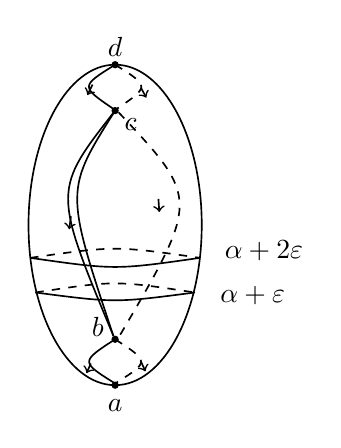
\begin{tikzpicture}[line width=0.6pt,scale=1.1]
  \draw (0,0) ellipse (1.0 and 1.85);
  \fill (0,1.85) circle (1.2pt);
  \fill (0,1.32) circle (1.2pt);
  \fill (0,-1.32) circle (1.2pt);
  \fill (0,-1.85) circle (1.2pt);
  \draw (0,1.85) .. controls (-0.40,1.60) .. (-0.02,1.34);
  \draw[->] (-0.26,1.62) -- (-0.32,1.50);
  \draw[dashed] (0,1.85) .. controls (0.40,1.60) .. (0.02,1.34);
  \draw[->] (0.30,1.58) -- (0.36,1.47);
  \draw (0,1.32) .. controls (-0.72,0.4) .. (-0.02,-1.28);
  \draw (0,1.32) .. controls (-0.58,0.4) .. (-0.02,-1.28);
  \draw[->] (-0.51,0.1) -- (-0.53,-0.05);
  \draw[dashed] (0.04,1.30) .. controls (0.98,0.3) .. (0.04,-1.30);
  \draw[->] (0.50,0.30) -- (0.51,0.15);
  \draw (0,-1.32) .. controls (-0.40,-1.58) .. (0,-1.83);
  \draw[->] (-0.28,-1.60) -- (-0.33,-1.71);
  \draw[dashed] (0,-1.32) .. controls (0.40,-1.58) .. (0,-1.83);
  \draw[->] (0.30,-1.58) -- (0.35,-1.69);
  \draw (-0.98,-0.38) .. controls (0,-0.52) .. (0.98,-0.38);
  \draw[dashed] (-0.98,-0.38) .. controls (0,-0.24) .. (0.98,-0.38);
  \draw (-0.92,-0.78) .. controls (0,-0.9) .. (0.92,-0.78);
  \draw[dashed] (-0.92,-0.78) .. controls (0,-0.64) .. (0.92,-0.78);
  \node at (0,2.06) {$d$};
  \node at (0.18,1.16) {$c$};
  \node at (-0.20,-1.18) {$b$};
  \node at (0,-2.08) {$a$};
  \node[right] at (1.15,-0.3) {$\alpha+2\varepsilon$};
  \node[right] at (1.1,-0.82) {$\alpha+\varepsilon$};
\end{tikzpicture}
\caption{}
\label{fig:torus-strip}
\end{minipage}\hfill
\begin{minipage}[b]{0.54\textwidth}
\centering
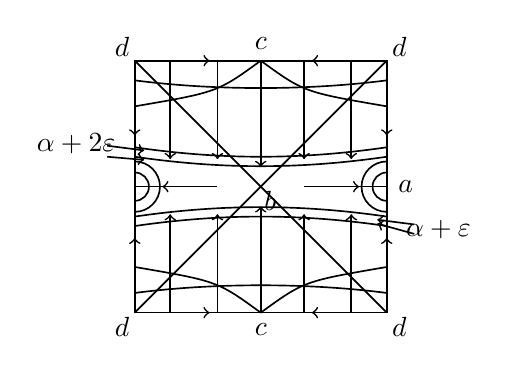
\begin{tikzpicture}[line width=0.6pt,scale=1.0]
  \draw (0,0) rectangle (3.2,3.2);
  \draw (0,1.6) -- (0.9,1.6); \draw[->] (1.05,1.6) -- (0.35,1.6);
  \draw (2.3,1.6) -- (3.2,1.6); \draw[->] (2.15,1.6) -- (2.85,1.6);
  \draw (1.6,3.2) -- (1.6,2.0); \draw[->] (1.6,2.15) -- (1.6,1.85);
  \draw (1.6,1.2) -- (1.6,0); \draw[->] (1.6,1.05) -- (1.6,1.35);
  \foreach \x in {0.45,1.05,2.15,2.75}{
    \draw (\x,3.2) -- (\x,2.5); \draw[->] (\x,2.5) -- (\x,1.95);
    \draw (\x,0) -- (\x,0.7); \draw[->] (\x,0.7) -- (\x,1.25);
  }
  \draw (1.6,1.6) -- (0,3.2);
  \draw (1.6,1.6) -- (3.2,3.2);
  \draw (1.6,1.6) -- (0,0);
  \draw (1.6,1.6) -- (3.2,0);
  \draw (0,1.92) arc (90:-90:0.32);
  \draw (0,1.78) arc (90:-90:0.18);
  \draw (3.2,1.92) arc (90:270:0.32);
  \draw (3.2,1.78) arc (90:270:0.18);
  \draw (1.6,3.2) .. controls (1.05,2.8) .. (0,2.62);
  \draw (1.6,3.2) .. controls (2.15,2.8) .. (3.2,2.62);
  \draw (1.6,0) .. controls (1.05,0.4) .. (0,0.58);
  \draw (1.6,0) .. controls (2.15,0.4) .. (3.2,0.58);
  \draw (0,2.95) .. controls (1.0,2.82) and (2.2,2.82) .. (3.2,2.95);
  \draw (0,0.25) .. controls (1.0,0.38) and (2.2,0.38) .. (3.2,0.25);
  \draw (-0.0,2.1) .. controls (1.1,1.94) and (2.1,1.94) .. (3.2,2.1);
  \draw (0,1.98) .. controls (1.1,1.82) and (2.1,1.82) .. (3.2,1.98);
  \draw (0,1.22) .. controls (1.1,1.38) and (2.1,1.38) .. (3.2,1.22);
  \draw (0,1.1) .. controls (1.1,1.26) and (2.1,1.26) .. (3.2,1.1);
  \node[left] at (-0.12,2.15) {$\alpha+2\varepsilon$};
  \draw[->] (-0.35,2.12) -- (0.12,2.06);
  \draw[->] (-0.35,1.98) -- (0.12,1.94);
  \node[right] at (3.32,1.05) {$\alpha+\varepsilon$};
  \draw[->] (3.55,1.12) -- (3.08,1.18);
  \draw[->] (3.55,1.0) -- (3.08,1.13);
  \draw[->] (0.55,3.2) -- (0.95,3.2);
  \draw[->] (2.65,3.2) -- (2.25,3.2);
  \draw[->] (0.55,0) -- (0.95,0);
  \draw[->] (2.65,0) -- (2.25,0);
  \draw[->] (0,2.65) -- (0,2.25);
  \draw[->] (0,0.55) -- (0,0.95);
  \draw[->] (3.2,2.65) -- (3.2,2.25);
  \draw[->] (3.2,0.55) -- (3.2,0.95);
  \node at (-0.16,3.38) {$d$};
  \node at (1.6,3.42) {$c$};
  \node at (3.36,3.38) {$d$};
  \node at (3.44,1.6) {$a$};
  \node at (1.72,1.42) {$b$};
  \node at (-0.16,-0.18) {$d$};
  \node at (1.6,-0.22) {$c$};
  \node at (3.36,-0.18) {$d$};
\end{tikzpicture}
\caption{}
\label{fig:square-strip}
\end{minipage}
\end{figure}

\trCriticalPoint{} $b$ 的一个\trMorse{}邻域在\cref{fig:square-strip}的中部清晰可见。我们把它从这幅图中提取出来（\cref{fig:extract-model}），并在模型有用的那一部分里修改\trVectorField（\cref{fig:modification-model}）。这最后一幅图画的是与\cref{fig:model}相同的模型，即 $Q\times D^k\times[0,m]$，只不过此时 $Q$ 是维数为 $n-k-1=0$ 的\trSphere，而 $D^k$ 是维数为 $k=1$ 的\trDisk。

\begin{figure}[htbp]
\begin{minipage}[b]{0.50\textwidth}
\centering
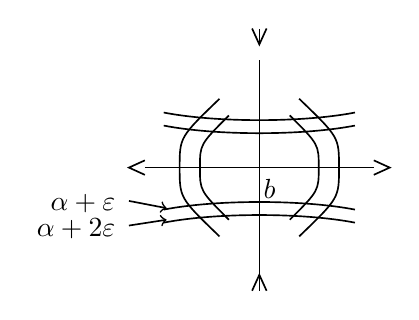
\begin{tikzpicture}[line width=0.6pt,scale=0.92]
  \draw (0,-1.7) -- (0,1.48);
  \draw (0.1,-1.7) -- (0,-1.48) -- (-0.1,-1.7);
  \draw (0,1.7) -- (0,1.92);
  \draw (-0.1,1.92) -- (0,1.7) -- (0.1,1.92);
  \draw (-1.58,0) -- (1.58,0);
  \draw (-1.58,-0.1) -- (-1.8,0) -- (-1.58,0.1);
  \draw (1.58,-0.1) -- (1.8,0) -- (1.58,0.1);
  \draw (-0.55,0.95) .. controls (-1.1,0.42) .. (-1.1,0)
        .. controls (-1.1,-0.42) .. (-0.55,-0.95);
  \draw (-0.42,0.72) .. controls (-0.82,0.32) .. (-0.82,0)
        .. controls (-0.82,-0.32) .. (-0.42,-0.72);
  \draw (0.55,0.95) .. controls (1.1,0.42) .. (1.1,0)
        .. controls (1.1,-0.42) .. (0.55,-0.95);
  \draw (0.42,0.72) .. controls (0.82,0.32) .. (0.82,0)
        .. controls (0.82,-0.32) .. (0.42,-0.72);
  \draw (-1.32,0.58) .. controls (-0.6,0.44) and (0.6,0.44) .. (1.32,0.58);
  \draw (-1.32,0.76) .. controls (-0.6,0.62) and (0.6,0.62) .. (1.32,0.76);
  \draw (-1.32,-0.58) .. controls (-0.6,-0.44) and (0.6,-0.44) .. (1.32,-0.58);
  \draw (-1.32,-0.76) .. controls (-0.6,-0.62) and (0.6,-0.62) .. (1.32,-0.76);
  \node at (0.14,-0.3) {$b$};
  \node[left] at (-1.85,-0.5) {$\alpha+\varepsilon$};
  \draw[->] (-1.8,-0.46) -- (-1.28,-0.56);
  \node[left] at (-1.85,-0.85) {$\alpha+2\varepsilon$};
  \draw[->] (-1.8,-0.8) -- (-1.28,-0.72);
\end{tikzpicture}
\caption{模型的截取部分}
\label{fig:extract-model}
\end{minipage}\hfill
\begin{minipage}[b]{0.46\textwidth}
\centering
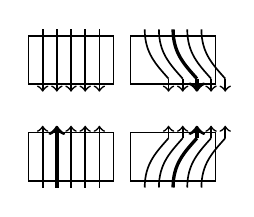
\begin{tikzpicture}[line width=0.6pt,scale=0.72]
  \draw (0,0.85) rectangle (1.5,1.7);
  \foreach \x in {0.25,0.5,0.75,1.0,1.25}{ \draw (\x,1.82) -- (\x,1.0); \draw[->] (\x,1.0) -- (\x,0.72); }
  \draw (1.8,0.85) rectangle (3.3,1.7);
  \foreach \x in {2.05,2.3,2.8,3.05}{ \draw (\x,1.82) .. controls (\x,1.4) and (\x+0.2,1.2) .. (\x+0.42,0.95); \draw[->] (\x+0.42,0.95) -- (\x+0.42,0.72); }
  \draw[line width=1.2pt] (2.55,1.82) .. controls (2.55,1.4) and (2.75,1.2) .. (2.97,0.95);
  \draw[->,line width=1.2pt] (2.97,0.95) -- (2.97,0.72);
  \draw (0,-0.85) rectangle (1.5,0);
  \foreach \x in {0.25,0.75,1.0,1.25}{ \draw (\x,-0.97) -- (\x,-0.15); \draw[->] (\x,-0.15) -- (\x,0.12); }
  \draw[line width=1.2pt] (0.5,-0.97) -- (0.5,-0.15); \draw[->,line width=1.2pt] (0.5,-0.15) -- (0.5,0.12);
  \draw (1.8,-0.85) rectangle (3.3,0);
  \foreach \x in {2.05,2.3,2.8,3.05}{ \draw (\x,-0.97) .. controls (\x,-0.55) and (\x+0.2,-0.35) .. (\x+0.42,-0.1); \draw[->] (\x+0.42,-0.1) -- (\x+0.42,0.12); }
  \draw[line width=1.2pt] (2.55,-0.97) .. controls (2.55,-0.55) and (2.75,-0.35) .. (2.97,-0.1);
  \draw[->,line width=1.2pt] (2.97,-0.1) -- (2.97,0.12);
\end{tikzpicture}
\caption{模型中的修改}
\label{fig:modification-model}
\end{minipage}
\end{figure}

把这一修改放回曲面中去，便给出一个具有预期性质的\trVectorField（\cref{fig:modified-field}）。

\begin{figure}[htbp]
\centering
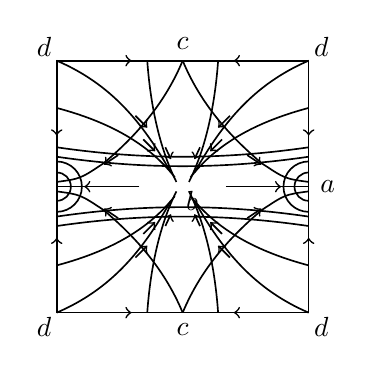
\begin{tikzpicture}[line width=0.6pt,scale=1.0]
  \draw (0,0) rectangle (3.2,3.2);
  \draw (0,1.6) -- (0.9,1.6); \draw[->] (1.05,1.6) -- (0.35,1.6);
  \draw (2.3,1.6) -- (3.2,1.6); \draw[->] (2.15,1.6) -- (2.85,1.6);
  \draw (0,1.92) arc (90:-90:0.32);
  \draw (0,1.78) arc (90:-90:0.18);
  \draw (3.2,1.92) arc (90:270:0.32);
  \draw (3.2,1.78) arc (90:270:0.18);
  \draw (0,2.1) .. controls (1.1,1.94) and (2.1,1.94) .. (3.2,2.1);
  \draw (0,1.98) .. controls (1.1,1.82) and (2.1,1.82) .. (3.2,1.98);
  \draw (0,1.22) .. controls (1.1,1.38) and (2.1,1.38) .. (3.2,1.22);
  \draw (0,1.1) .. controls (1.1,1.26) and (2.1,1.26) .. (3.2,1.1);
  \draw[->] (0.55,3.2) -- (0.95,3.2);
  \draw[->] (2.65,3.2) -- (2.25,3.2);
  \draw[->] (0.55,0) -- (0.95,0);
  \draw[->] (2.65,0) -- (2.25,0);
  \draw[->] (0,2.65) -- (0,2.25);
  \draw[->] (0,0.55) -- (0,0.95);
  \draw[->] (3.2,2.65) -- (3.2,2.25);
  \draw[->] (3.2,0.55) -- (3.2,0.95);
  \draw (1.6,3.2) .. controls (1.35,2.6) and (0.95,2.2) .. (0.6,1.9)
        .. controls (0.3,1.7) .. (0,1.66);
  \draw[->] (0.78,2.0) -- (0.6,1.88);
  \draw (1.6,3.2) .. controls (1.85,2.6) and (2.25,2.2) .. (2.6,1.9)
        .. controls (2.9,1.7) .. (3.2,1.66);
  \draw[->] (2.42,2.0) -- (2.6,1.88);
  \draw (1.6,0) .. controls (1.35,0.6) and (0.95,1.0) .. (0.6,1.3)
        .. controls (0.3,1.5) .. (0,1.54);
  \draw[->] (0.78,1.2) -- (0.6,1.32);
  \draw (1.6,0) .. controls (1.85,0.6) and (2.25,1.0) .. (2.6,1.3)
        .. controls (2.9,1.5) .. (3.2,1.54);
  \draw[->] (2.42,1.2) -- (2.6,1.32);
  \draw (1.15,3.2) .. controls (1.2,2.5) and (1.35,2.0) .. (1.52,1.66);
  \draw[->] (1.38,2.1) -- (1.45,1.95);
  \draw (2.05,3.2) .. controls (2.0,2.5) and (1.85,2.0) .. (1.68,1.66);
  \draw[->] (1.82,2.1) -- (1.75,1.95);
  \draw (1.15,0) .. controls (1.2,0.7) and (1.35,1.2) .. (1.52,1.54);
  \draw[->] (1.38,1.1) -- (1.45,1.25);
  \draw (2.05,0) .. controls (2.0,0.7) and (1.85,1.2) .. (1.68,1.54);
  \draw[->] (1.82,1.1) -- (1.75,1.25);
  \draw (0,3.2) .. controls (0.7,2.9) and (1.1,2.4) .. (1.45,1.78);
  \draw[->] (1.0,2.5) -- (1.15,2.35);
  \draw (3.2,3.2) .. controls (2.5,2.9) and (2.1,2.4) .. (1.75,1.78);
  \draw[->] (2.2,2.5) -- (2.05,2.35);
  \draw (0,0) .. controls (0.7,0.3) and (1.1,0.8) .. (1.45,1.42);
  \draw[->] (1.0,0.7) -- (1.15,0.85);
  \draw (3.2,0) .. controls (2.5,0.3) and (2.1,0.8) .. (1.75,1.42);
  \draw[->] (2.2,0.7) -- (2.05,0.85);
  \draw (0,2.6) .. controls (0.75,2.4) and (1.2,2.1) .. (1.5,1.72);
  \draw[->] (1.1,2.2) -- (1.25,2.05);
  \draw (3.2,2.6) .. controls (2.45,2.4) and (2.0,2.1) .. (1.7,1.72);
  \draw[->] (2.1,2.2) -- (1.95,2.05);
  \draw (0,0.6) .. controls (0.75,0.8) and (1.2,1.1) .. (1.5,1.48);
  \draw[->] (1.1,1.0) -- (1.25,1.15);
  \draw (3.2,0.6) .. controls (2.45,0.8) and (2.0,1.1) .. (1.7,1.48);
  \draw[->] (2.1,1.0) -- (1.95,1.15);
  \node at (-0.16,3.38) {$d$};
  \node at (1.6,3.42) {$c$};
  \node at (3.36,3.38) {$d$};
  \node at (3.44,1.6) {$a$};
  \node at (1.72,1.42) {$b$};
  \node at (-0.16,-0.18) {$d$};
  \node at (1.6,-0.22) {$c$};
  \node at (3.36,-0.18) {$d$};
\end{tikzpicture}
\caption{修改后的场}
\label{fig:modified-field}
\end{figure}
